\documentclass[a4paper]{report}
\usepackage[T1]{fontenc}
\usepackage[french]{babel}
\usepackage{setspace}
\usepackage{graphicx}
\usepackage{wrapfig}
\usepackage{lscape}
\usepackage{bookmark}
\usepackage{rotating}
\usepackage{subcaption}
\usepackage{float}
\usepackage{eurosym}
\usepackage[headheight=13pt,top=3cm, bottom=2cm, left=1cm, right=1cm]{geometry}
\usepackage{pdfpages}
\usepackage{fancyhdr}
\pagestyle{fancy}
\usepackage{hyperref}
\hypersetup{
    colorlinks=true,
    linkcolor=black,
    citecolor=black,
    filecolor=black,
    urlcolor=black,
}
\usepackage{array,multirow,makecell}
\setcellgapes{3pt}
\setlength{\parindent}{1.1cm}
\makegapedcells
\newcolumntype{L}[1]{>{\raggedright\arraybackslash}b{#1}}
\newcolumntype{R}[1]{>{\raggedleft\arraybackslash}b{#1}}
\newcolumntype{C}[1]{>{\centering\arraybackslash}b{#1}}
\renewcommand{\footrulewidth}{1pt}
\fancyfoot[L]{ENSIAS}
\fancyfoot[C]{\textbf{\thepage}}
\fancyfoot[R]{Année universitaire: 2020/2021}
\begin{document}
\begin{titlepage}
	\begin{center}
		\begin{figure}[!h]
			\vspace{- 2 cm}
			\hspace{ 0 cm}
			
\includegraphics[width=9em]{images/ensias.jpeg}
		\end{figure}
		\begin{figure}[!h]
			\vspace{- 3.34cm}
			\hspace{14 cm}
			
\includegraphics[width=10em]{images/um5.jpeg}
		\end{figure}
	\end{center}

	\begin{center}
		\noindent \hspace{ 0.3 cm }\Huge \textbf{Rapport de Stage Fin de
			deuxième Année}
		\vspace*{0.1cm}

		\vspace*{0.1cm}
		\begin{center}
			\rule{0.9\linewidth}{1pt}
		\end{center}
		\begin{center}
			\noindent \hspace{ 0.4 cm}{\large \textsc{ Création d'une
					plateforme Web pour la gestion et le suivi des contrats du transport
					délégués}}\\
		\end{center}

		\vspace*{0.5cm} \noindent \hspace{ -0.5 cm} \large
		\begin{figure}[H]
			\begin{center}
				
\includegraphics[scale=0.8]{images/logo-uir2.jpg}
			\end{center}
		\end{figure}
		\raggedright
		{\textbf{\emph{Préparé par: KOTBI Abderrahamane}}}
		\raggedleft\rule{0.7\linewidth}{2pt}\\
		\raggedleft{\textbf{\emph{Membres de Jury: *****}}}\\
		\Large\emph{Année universitaire: 2020-2021}

	\end{center}
\end{titlepage}
\pagenumbering{arabic} \setcounter{page}{1}
\addcontentsline{toc}{chapter}{Remerciements}
\begin{doublespace}
	\begin{center}
		\vspace*{1cm}

		\textbf{\huge{Remerciements}}

	\end{center}

	\textit{
		Avant d'aborder la description des parties importantes du projet,
		j'aimerai tout d’abord exprimer ma gratitude
		intense à toute personne qui a contribué énormément dans l'élaboration
		et la réalisation de ce travail. Je commence
		ainsi par offrir mes remerciements à l'intégralité des personnes
		travaillant au sein de l’école Nationale supérieure d’informatique et d’analyse
		des systèmes. Ces bonnes hommes et femmes qui ne cessent de nous préparer, moi
		et
		mes collègues, pour de telles expériences afin de bien s’intégrer dans
		le cadre réelle du marché de travail.
		Toute ma gratitude et profonde reconnaissance s’adressent à à tous mes
		encadrants de stages: Mme.\textbf{***f***} ****,
		M..\textbf{***m***} ****   . Je vous remercie énormément pour m'avoir
		garanti un encadrement de qualité pour bien mener
		et assurer la réalisation de ce travail dans les meilleures des
		conditions.
	}


	\clearpage
	\addcontentsline{toc}{chapter}{Résumé}
	\begin{center}
		\vspace*{1cm}

		\textbf{\huge{Résumé}}

	\end{center}
	Ce document représente une étude synthétique du travail réalisé dans le
	cadre de mon stage d'été de deuxième année. J'ai effectué mon stage au sein de
	l'université internationale de Rabat \textbf{UIR}. Ce dernier a duré les deux
	mois juillet et août de l'année 2021. L’objectif principal de ce travail
	consiste à développer une plateforme Web pour la gestion et le suivi des
	contrats du transport délégués. D'ailleurs, le travail effectué dans le cadre
	de ce projet m'a représenté la bonne chance pour appliquer mes savoirs et
	savoirs-faire acquis durant cette année. En ce sens, la réalisation du projet a
	passé en trois étapes principal: l'élaboration d'une analyse détaillée des
	besoins du client, conception des différentes composantes de l'application, et
	enfin l'implémentation des objectifs soulignés. Par conséquent, j'ai eu la
	chance d'utiliser plusieurs technologies, outils et concepts qui m'ont aidé à
	développer cette solution.

	Le reste de ce rapport est organisé comme suit : le chapitre I est dédié à
	la présentation de
	l’organisme d’accueil et du client. Quant au chapitre II, il traite
	l’analyse du problème ainsi que la spécification des besoins. Ensuite le
	chapitre III présente l´étude conceptuelle. Enfin le chapitre IV traite la
	partie réalisation.

	\textbf	{\\Mots clés :\\ Gestion, Suivi, Donnée, Contrats délégués,
		Transport urbain, Centralisation, Application low-code.}

	\clearpage
	\addcontentsline{toc}{chapter}{Abstract}
	\begin{center}
		\vspace*{1cm}
		\textbf{\huge{Abstract}}
	\end{center}

	This document represents a synthetic study of the work carried out as part
	of my second-year summer intern-ship.
	I did my intern-ship at the international university of Rabat \textbf{UIR}.
	The latter lasted the two months
	July and August of the year 2021. It aims to develop a web platform for the
	management and monitoring of
	delegated transport contracts. Moreover, the work carried out in this
	project represented good opportunity
	for me to apply and sharpen my skills and my knowledge acquired during this
	year. Thus, the realization
	of the project has gone through three main stages: the extraction of a
	detailed analysis of the client's
	needs, the design of the application's different components, and finally
	the implementation of the outlined objectives.
	Therefore, I had the chance to use several technologies, tools, and
	concepts that helped me develop this solution.

	\textbf{\\Keywords:\\Management, Monitoring, Data, Delegated contracts,
		Urban transport, Centralization, Low-code application.}
\end{doublespace}

\newpage

\renewcommand{\contentsname}{Table de matières}
\setcounter{tocdepth}{4}
\tableofcontents

\cleardoublepage

\addcontentsline{toc}{chapter}{\listfigurename}
\listoffigures
\newpage
\begin{doublespace}
	\addcontentsline{toc}{chapter}{Introduction générale}
	\begin{center}
		\vspace*{1cm}
		\textbf{\huge{Introduction générale}}
	\end{center}
	\renewcommand{\headrulewidth}{1pt}
	\fancyhead[R]{\textbf{Introduction générale}}
	\fancyhead[L]{\hspace*{5cm}}
	Dans le cadre de la modernisation de la gestion des secteurs publics
	collectifs
	marocains, l’état a créé des contrats de gestion déléguées. Parmi ces
	dernières, les
	contrats de gestion de transport urbain. Placer le citoyen au cœur des
	politiques et
	services publics en constitue un objectif fondamentale. En conséquence, le
	contrat
	vise à assurer des services publics de qualité, accessibles à tous les
	citoyens sans discrimination, à des coûts maitrisés tenant compte du
	pouvoir
	d’achat. D'où  l'importance de la bonne gestion et le suivi de ces
	contrats, pour garder
	les droits et les attentes de la population.
	Par ailleurs, l’état a pris ce sens pour réaliser ses objectifs d’ouverture
	sur l’économie
	mondiale, le soutien des entreprises publiques, et l’amélioration de ses
	services.
	En parallèle avec ceci, l’état a essayé de gagner les défis de la
	régionalisation.
	Par conséquent, la gestion et le suivis des contrats de transport a devenu
	une tâche
	fondamentale. Or, effectuer cette tâche en utilisant la méthode classique,
	par plusieurs documents,
	ne représente plus une bonne solution, vue le nombre de lecture et de
	vérification
	des données importantes dans les documents nombreux. En plus, cela ne
	permet pas d’en
	tirer profits pour prendre les bons décisions facilement. Ainsi, je propose
	une
	solution simple pour la gestion et la représentation des données en
	question.
	\newpage
	\chapter{Cadre générale du projet}
	\renewcommand{\headrulewidth}{1pt}
	\fancyhead[R]{\textbf{Chapitre \thechapter: Cadre générale du projet}}
	\fancyhead[L]{\hspace*{5cm}}
	Dans ce chapitre j'entame le projet dans son cadre général : présentation
	de l’organisme d’accueil \textbf{UIR},
	et de client, présentation de l'idée de l'application, présentation du
	contexte du projet, de la problématique et des objectifs fixés,
	et de la démarche de la réalisation que j'ai adopté.
	\section{Présentation de l’organisme d’accueil}
	\subsection{UIR}

	L’Université Internationale de Rabat ou \textbf{UIR} est une université
	privée fondée en 2010 sous contrat avec l’État marocain.
	L'\textbf{UIR} concrétise ainsi le premier partenariat public-privé dans le
	domaine de l'enseignement supérieur au Maroc.
	Poursuivant l'objectif d'accompagner le Royaume du Maroc dans son
	développement, l'\textbf{UIR} a développé un catalogue
	de formation de haut niveau en adéquation avec les différentes stratégies
	impulsées par le Maroc (Plan solaire marocain
	, plan d'accélération industrielle, plan de digitalisation, etc.). Surtout
	sur le plan informatique, l'\textbf{UIR} demeure
	un partenaire important de l'état. Elle a plusieurs contributions en terme
	d'éducation et de préparation des cadres, ainsi
	qu'en terme de consulting, de recherche, de résolutions des problèmes
	émergents, et en terme d’innovation.
	\begin{figure}[H]
		\begin{center}
			
\includegraphics[scale=0.1]{images/logo-uir.jpg}
			\caption{Organisme d'acceuil}
		\end{center}
	\end{figure}
	\subsection{Partenaire de consulting technique: Dyn IT}

	\textbf{DYN IT MAROC} est le résultat de l’expérience de plusieurs
	Consultants en IT et Education.
	Nous conseillons et proposons des services en Ingénierie Informatique.
	Notre mission est de
	vous faire collaborer efficacement. Elle s'engage à aider leurs clients
	en fournissant des solutions de collaboration flexibles, évolutives et
	surtout abordables.
	Elle offrent des services de consultation et de formation en technologies
	Microsoft. En fait, \textbf{DYN IT} est un partenaire Microsoft.
	\begin{figure}[H]
		\begin{center}
			
\includegraphics[scale=0.6]{images/dynit.png}
			\caption{Organisme d'acceuil}
		\end{center}
	\end{figure}
	\section{Présentation du Client}

	La Direction Générale des Collectivités Territoriales \textbf{DGCT} est
	chargée de la préparation des décisions du ministre de l’Intérieur,
	dans le cadre des attributions qui lui sont conférées en vertu des textes
	législatifs et réglementaires relatifs aux collectivités
	territoriales, et du suivi de leur exécution. Elle assure également l’appui
	et l'accompagnement juridique, technique et financier
	des collectivités territoriales, des instances qui en relèvent, des
	établissements de coopération intercommunale et des groupements
	des collectivités territoriales. Elle est chargée également, en
	coordination avec les départements et organismes concernés, de
	concourir au développement territorial. Bref, ses missions sont en gros:
	\begin{itemize}
		\item Planification et développement territorial.
		\item Assistance des réseaux publics locaux, et des institutions
		      locales.
		\item Suivi juridique et gestion des services locaux.
		\item Amélioration de la mobilité urbaine et du transport.
		\item Développement des compétences et transformation digitale.
		\item Accompagnement financier des collectivités territoriales.
		\item Coopération décentralisée.
	\end{itemize}
	\begin{figure}[H]
		\begin{center}
			
\includegraphics[scale=0.27]{images/logo-fr.png}
			\caption{Client}
		\end{center}
	\end{figure}
	\newpage
	\section{Problématique}

	Dans le cadre de la bon gestion de territoire et des aménagements publics,
	plusieurs
	contrats de gestion déléguée du transport urbain sont signés. Ces derniers
	comportent
	plusieurs actes qui forment un ensemble de règles à respecter entre un
	délégant qui
	sont une ou plusieurs communes et un délégataire qui est une société. En
	addition,
	des pénalités sont imposées en cas de non respect des règles posées dans le
	contrat.
	Par conséquent, le suivi de la réalisation et du respect de ses actes est
	un devoir
	juridique. D’où l'importance d'avoir une solution pertinente pour veiller
	sur le
	respect des conditions prédéfinis.
	\\\textbf{Alors, comment peut on améliore les opérations de suivis et de
		traitements des données en questions?}
	\section{Solution et Objectifs du projet}

	La première étape de la conduite de projet est sans doute la plus évidente,
	mais peut-être
	aussi la plus cruciale. En effet, sans objectifs bien définis, il est
	difficile de savoir où votre projet
	va vous mener. Pour cela, avant de commencer dans la conception et la
	réalisation de ce projet,
	il faut tout d’abord fixer l’objectif principal de manière à développer la
	ligne d’actions à mener.
	Je cherche à concevoir et construire une application Web qui permet de
	saisir, d'enregistrer,
	et de traiter les données qui concernent les contrats de gestion de
	transport. La
	solution proposée est composée de deux partie: une première partie qui
	concerne la
	saisi et l'enregistrement des données sous la forme d'une plateforme web
	liée à une
	base de donné, et une deuxième partie qui concerne l'analyse des données.
	Bref, je cherche une solution pour:
	\begin{itemize}
		\item Centraliser l’information contenue dans les contrats de gestion
		      déléguée et
		      leurs avenants le cas échéant.
		\item Centraliser les documents exigés par le contrat que l’opérateur
		      est tenu de
		      fournir périodiquement à l’autorité délégante.
		\item Permettre aux utilisateurs de partager en interne des
		      informations et des
		      documents.
		\item Assurer le suivi de la gestion des contrats de transport urbain.
	\end{itemize}
	\section{Récapitulatif}
	Dans ce chapitre introductif, j'ai pu décrire le conteste général du
	projet, et
	déterminer son objectif principal. En addition, les aspects que je vais
	avoir besoin lors de la réalisation de cette application.
	Le chapitre qui suit consiste la phase d'analyse des besoins du projet.
	\newpage
	\chapter{Analyse}
	\renewcommand{\headrulewidth}{1pt}
	\fancyhead[R]{\textbf{Chapitre \thechapter: Analyse et conception}}
	\fancyhead[L]{\hspace*{5cm}}

	Ce chapitre représente le point de départ de mon travail. Premièrement,
	j'analyse et
	je spécifie les besoins du projet. Ensuite, j'identifie les différents
	acteurs. Et enfin, je
	modélise le tout dans un diagramme des cas d’utilisation général qui
	sera notre file conducteur
	durant la prochaine phase.
	\section{Étude du projet}
	\subsection{Introduction à l'analyse}
	Certes, la gestion et le suivis des données en utilisant des solutions
	Web ne date pas d'hier. Mais,
	elle demeure une solution optimisant en terme de temps et de
	productivité. Surtout,
	dans un tel cas où les informations sont, à la fois, cruciales et
	nombreuses. Ainsi, la solution proposée premièrement par la \textbf{DGST} est
	d'avoir une plateforme Web pour faciliter la collecte,
	le traitement, la présentation, et la centralisation de l'information.
	Sur la même longueur d'onde, j'ai
	travaillé sur la solution proposée avec une équipe de la \textbf{DGST}
	pour apporter les bonnes
	fonctionnalités répondantes aux besoins de cette dernière.
	\subsection{Description générale du projet}
	D'un point de vue technique le projet est décomposé en trois partie. La
	première concernant la partie client dans laquelle l'utilisateur peut saisir
	les données. Ensuite, une base de données et enfin la partie reporting.
	\begin{figure}[H]
		\begin{center}
			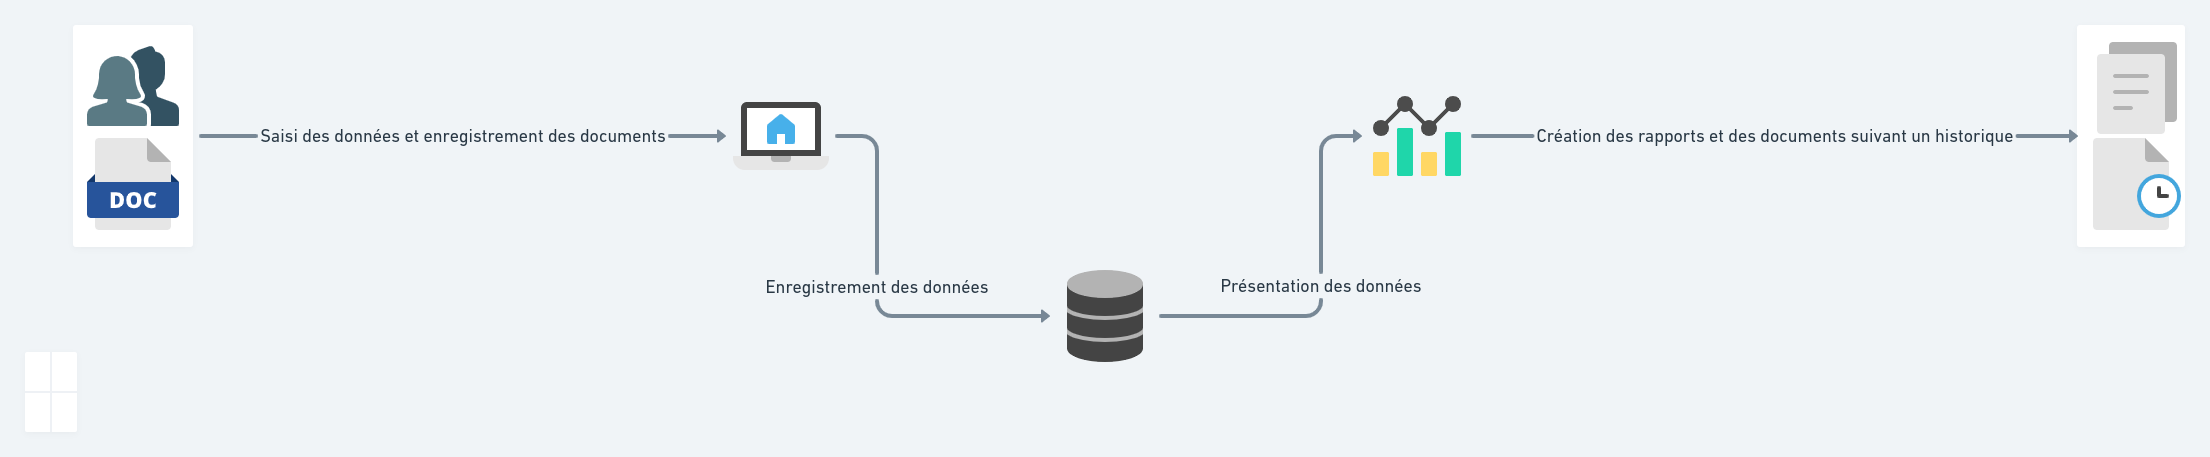
\includegraphics[scale=0.2]{images/pre-descip-projet.png}
			\caption{Description préliminaire du projet}
		\end{center}
	\end{figure}
	\subsection{Étude de l’existant}
	Après la recherche et des exemples similaire à notre projet, on a
	trouvé une diversité des sites web et des applications dédiées à la gestion et
	au suivi.
	À titre d'exemple on peut considérer l'application \textbf{\large Ecan}:\\
	Généralement, les applications similaires sont des applications qui
	aide à la gestion de donnée et des ressources, et la prise des décisions.
	L’application \emph{Environnement Canterbury (ECan)} fait partie du
	gouvernement local de la région de Canterbury en Nouvelle-Zélande. Ils ont
	utilisé la plate-forme \emph{Power
		(PowerApps, Microsoft Flow et Power BI)} pour gérer et rendre compte
	efficacement des projets d'eau douce et de ressources naturelles.\\
	D’après l'article intitulé Environnement Canterbury accélère le suivi
	des
	résultats avec \emph{la Power Platform} :
	"Environnement Canterbury travaille en partenariat avec les communautés
	de
	Canterbury pour promouvoir la gestion durable des ressources
	naturelles. Cela
	implique l'utilisation de méthodes innovantes, rentables et
	techniquement
	excellentes, et garantit que la prise de décision est basée sur des
	informations
	de la plus haute qualité. Ils travaillent sur des programmes de
	résultats
	environnementaux à long terme qui consistent en plusieurs étapes et
	projets
	connexes. ECan avait besoin d'une solution abordable qui offrirait une
	plus
	grande cohérence entre les projets, des niveaux de visibilité plus
	élevés et un
	accès plus rapide aux données."
	\begin{figure}[H]
		\begin{center}
			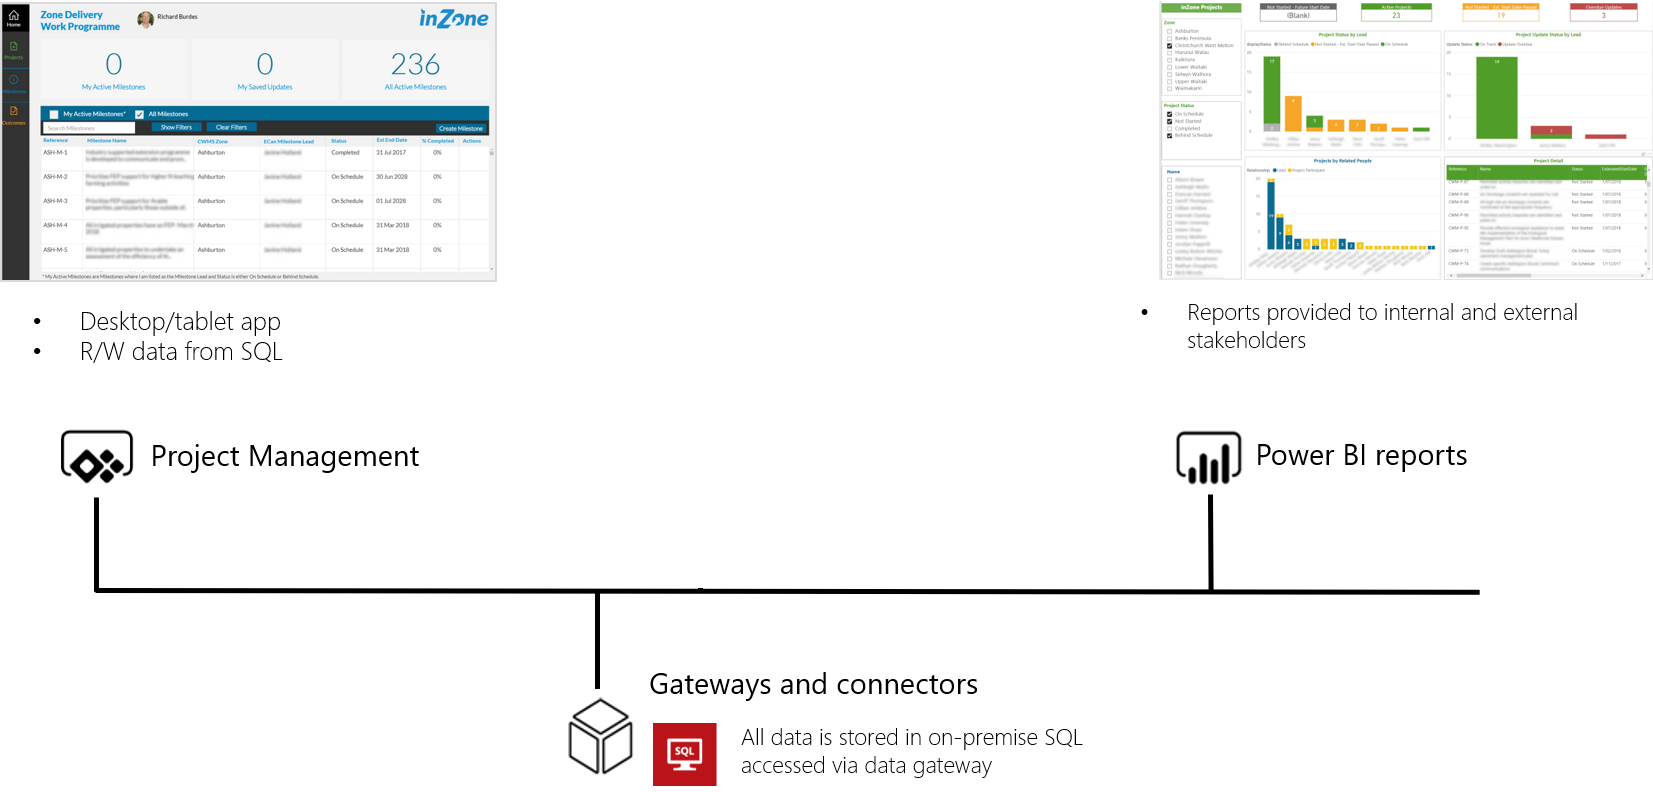
\includegraphics[scale=0.32]{images/example.png}
			\caption{Exemple de Environnement Canterbury (ECan)}
		\end{center}
	\end{figure}
	\newpage
	\section{Spécification des besoins}

	\subsection{Spécification des acteurs}
	Vu que les informations gérées par cette application sont des informations confidentielles de l'état, l'application va avoir en général un seul acteur:
	L'administrateur est la personne chargée de charger les informations des différentes communes et de gérer leurs données, préparées par les différentes communes du Maroc.
	\subsection{Besoins fonctionnels}
	\begin{itemize}
		\item Gestion des délégants et des délégataires: L'administrateur doit avoir
		      une section où il pourra gérer les délégants et les délégataires.
		\item Gestion des contrats: Il doit avoir également la possibilité de gérer les contrats signés. En addition, il peut suivre les avenants et les révisions de chaque contrats. Ainsi que le status de chaque avenant ou révision.
		\item Gestion des Avancements: L'application doit permettre de gérer les avancements semestriels des contrats. Aussi, consulter et suivre les changements apportés à chaque période.
		\item Présentation des tableaux de bord: L'application doit présenter des données historisées de chaque contrats permettant de bien estimer la qualité de service en question et prendre les bonnes décisions.
	\end{itemize}
	\subsection{Les besoins non fonctionnels}
	Les besoins fonctionnels sont basiques pour un fonctionnement
	correcte et une réponse fiable aux besoins des utilisateurs, mais il y a des
	autres besoins qui tendent à améliorer la performance et la qualité de
	l'application pour une utilisation plus adéquate.
	\begin{itemize}
		\item Fiabilité de la plateforme: L’application doit
		      fonctionner sans erreur.
		\item Ergonomie, souplesse et confort d’utilisation: Pour
		      faciliter l’utilisation, notre plateforme doit offrir une interface unifiée,
		      conviviale et ergonomique.
		\item Gain de temps: L'application doit optimiser les
		      traitements pour avoir un temps de réponse minimale.
		\item Maintenabilité et sociabilité: La source de l'application doit être compréhensible
		      afin d’assurer son état évolutif et extensible par rapport aux besoins des utilisateurs. En outre, l’expérience des utilisateurs doit être meilleurs.
		\item Sécurité: Notre plateforme doit  être très authentique en ce qui concerne les informations confidentielles des communes.
	\end{itemize}
	\section{Analyse Fonctionnelle}
	Suivant à ce qui précède et d’après l’ensemble des documents communiqués par mes encadrants, j’ai essayé de créer une décomposition hiérarchique des fonctionnalités du projet.
	\begin{figure}[H]
		\begin{center}
			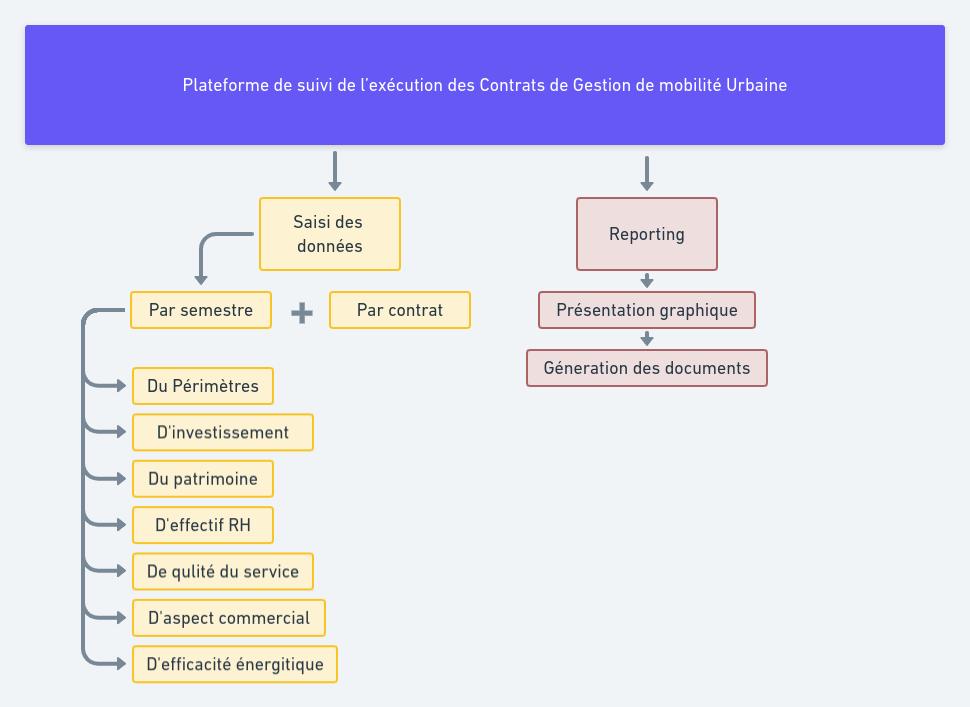
\includegraphics[scale=0.5]{images/WBS KPI.png}
			\caption{Décomposition fonctionnelle du projet}
		\end{center}
	\end{figure}
	Ainsi, J'ai divisé le projet en deux parties fondamentales. En plus, on peut voir clairement les grandes fonctionnalités demandées dans cette application. Par conséquent, l'application peut être divisée en deux partie: partie saisi et partie reporting.
	\begin{itemize}
		\item La partie saisi est la partie dans laquelle l'administrateur peut ajouter des délégants et des délégataires. En conséquences, il peut définir un contrat. Par ailleurs, le contrat définit peut avoir des mises à jour semestriels des informations qui le concerne.
		\item La partie reporting est la partie qui concerne les tableaux de bords de l’application. Il doit bien présenter les informations saisîtes. En plus, il est préférables d'avoir la possibilité de générer des documents contenants les informations saisîtes.
	\end{itemize}
	\section{Analyse technique}
	La solution que je propose est une solution basée sur les données.
	Autrement dite, elle permet à son utilisateur d'interagir avec plusieurs
	informations. En outre, elle représente une solution spécialisée pour
	l'acquisition, la gestion et la présentation d'informations. Ainsi, le groupe du projet à proposer l'ensemble des outils suivants:
	\begin{figure}[H]
		\begin{center}
			
\includegraphics[scale=0.41]{images/outilsDB.png}
			\caption{Décomposition hiérarchique orientée livrable du projet}
		\end{center}
	\end{figure}
	Microsoft SQL Server est un système de gestion
	de base de données relationnelle développé
	par Microsoft. En tant que serveur de base de
	données, il s'agit d'un produit logiciel dont la
	fonction principale est de stocker et de
	récupérer des données à la demande d'autres
	applications logicielles, qui peuvent
	s'exécuter sur le même ordinateur ou sur un
	autre ordinateur via un réseau.
	\begin{figure}[H]
		\begin{center}
			
\includegraphics[scale=0.41]{images/outilsDEV.png}
			\caption{Décomposition hiérarchique orientée livrable du projet}
		\end{center}
	\end{figure}
	Power Apps est un service permettant de créer
	et d'utiliser des applications professionnelles
	personnalisées qui se connectent à vos
	données et fonctionnent sur le Web et les
	appareils mobiles - sans le temps et les frais
	de développement de logiciels personnalisés.
	\begin{figure}[H]
		\begin{center}
			
\includegraphics[scale=1.1]{images/outilsREP.png}
			\caption{Décomposition hiérarchique orientée livrable du projet}
		\end{center}
	\end{figure}
	Power BI est un service d'analyse
	commerciale de Microsoft. Il vise à fournir des
	visualisations interactives et des capacités de
	business intelligence avec une interface
	suffisamment simple pour que les utilisateurs
	finaux puissent créer leurs propres rapports et
	tableaux de bord. Il fait partie de la plate-
	forme Microsoft Power.\\
	Suite à cette proposition le consultant technique a approuver ces choix. Ainsi la décision est prise d'utiliser ces technologies Microsoft afin de réaliser une application Low-Code pour la gestion des contrats de transport délégués.
	\section{Récapitulatif}
	
\end{doublespace}

\end{document}
